% Results. Every number: see paper/figs/README.md and paper/EVIDENCE.md (IDs in comments).
\section{Results}
\label{sec:results}

\subsection{C1: Uplink Queuing, Not Coverage, and an Autonomic Cap}
\label{sec:r-cap}

\textit{The long forest outages are a queue inside the UE.} With the four
robots parked under canopy (24--30\,dB uplink attenuation) and the UAV at
40\,m, C2 was clean without load. Once the four 1.5\,Mb/s video feeds started,
uplink ping RTT grew from about 60\,ms to minutes within the first seconds and
kept rising for the whole load period, peaking at 350--444\,s
(Fig.~\ref{fig:rtt}(a)); 64--91\,\% of pings were lost and, for 64\,\% of the
time, all eight probes (one per direction per robot) were lost at once (Table~\ref{tab:static}). Probes were
delayed rather than dropped, and the links drained only 0.13--0.49\,Mb/s of the
1.5\,Mb/s offered. The kernel queue on each robot's TUN interface held no backlog and dropped
nothing, so the excess was buffered beyond the kernel, inside the OAI UE
software (E1); we did not instrument which UE layer holds it. The drain rate is
not simply what the radio supports: in the capped placement runs the gNB's own
counters (modulation, code rate, allocated symbols) implied full-carrier uplink
rates of tens of Mb/s even in forest, far above 1.5\,Mb/s, and the emulator's
radio thread ran near one full core. Whether the limit is scheduling or
emulation is under measurement.
\todo{capacity sweep 0--35\,dB and 1/2/4-robot saturation, with gNB MAC
statistics and per-thread CPU (scheduled 15 Nov)} After the video stopped, C2 stayed dead for 14 to more than 18\,min,
consistent with each link slowly draining its backlog.

% E1: tab_static_load (analyse.py), ul_*.txt max RTT, CONGESTION_TEST_REPORT.md (qdisc); 79 MB figure removed (untraceable, review K6)
\begin{figure*}[t]
\centering
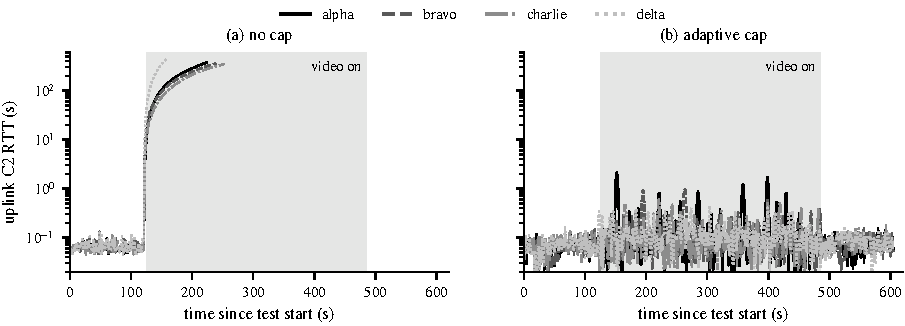
\includegraphics[width=\textwidth]{fig_rtt.pdf}
\caption{Uplink C2 ping RTT per robot in the static forest load test (log
scale; video on in the shaded interval). (a) Without a cap, RTT grows to
minutes; traces end where replies stop before the test ends. (b) With the
adaptive cap, RTT stays near its unloaded level.}
\label{fig:rtt}
\end{figure*}

\begin{table}[t]
\caption{Static Forest Load Test, Four Robots, 6\,min of Video}
\label{tab:static}
\centering
\footnotesize\setlength{\tabcolsep}{3pt}
% generated by tab_static_load.py -- do not edit
\begin{tabular}{@{}lccc@{}}
\toprule
 & No cap & Fixed 100\,kb/s & Adaptive \\
\midrule
Uplink ping loss, video on & 64--91\,\% & 0\,\% & 0\,\% \\
Uplink ping RTT, median & 3--4\,min & 69--87\,ms & 76--108\,ms \\
All probes lost (on / off) & 64 / 100\,\% & 0 / 0\,\% & 0 / 0\,\% \\
Recovery after video & 14--18+\,min & none & none \\
Video goodput (Mb/s) & 0.13--0.49 & 0.10 & 0.10--0.42 \\
Video latency, median & 2.2--2.8\,min & 1.08--1.11\,s & 0.30--1.08\,s \\
\bottomrule
\end{tabular}

\end{table}

\textit{Bounding the queue removes the outages.} A fixed 100\,kb/s cap below
every link's drain rate, applied at the same placement, removed all C2 loss and
the recovery tail, but discarded most of the video (Table~\ref{tab:static}).
The adaptive cap of Section~\ref{sec:cap} also gave zero C2 loss while settling
at a different rate on each link (medians 105--429\,kb/s, 32--40 cuts per robot
in 6\,min), delivering 0.10--0.42\,Mb/s of video at a median latency of
0.30--0.42\,s on three robots; the fourth, with the weakest link, ran at
1.08\,s, the time its 10-packet video queue takes to drain at about 100\,kb/s
(Fig.~\ref{fig:rtt}(b)). In open field, with 2--9\,dB of attenuation, every cap
rose to its 1.6\,Mb/s ceiling, made no cuts, and carried the full 1.55\,Mb/s
per robot at 82--89\,ms median latency (E4): in this test, where links were
strong, the cap stayed out of the way.
% E2, E3: cap_log.csv (medians, cuts), tab_static_load; E4: CONGESTION_TEST_REPORT follow-up 3

\textit{The cap lifts the like-for-like placement arms.} In a 30-min forest patrol with
the UAV hovering at 40\,m, the cap raised mean C2 availability from 66.8\,\% to
91.8\,\% against the same seed uncapped, cut the time with no robot connected
from 17.4\,\% to 0.9\,\%, and the 90th-percentile video latency from 73\,s to
1.6\,s (Table~\ref{tab:a5}). In the forest fly-off (Fig.~\ref{fig:caparms}), only arms A and B flew
the same policy with and without the cap: there, the time with no robot
connected fell from 25.4 and 25.9\,\% to 0.3 and 0.0\,\%, and mean C2 rose from
66.6 and 58.0\,\% to 89.1 and 88.9\,\%. Arms C and D also changed altitude
learner between the two conditions, so their improvement cannot be attributed
to the cap alone. Each comparison is one run per condition on different
nights, with no null control for those nights.

\textit{The cap turns minute-long outages into single missed cycles.} For the
same like-for-like runs, Fig.~\ref{fig:outage} gives the length of every C2
outage. Without the cap the median forest outage lasted 143\,s (arm A) and
97\,s (arm B), and 64\,\% and 59\,\% of outages exceeded a minute; with it
the medians fell to 17\,s and 19\,s and 11\,\% and 19\,\% exceeded a minute.
In open field the median fell from 48\,s to 11\,s (Table~\ref{tab:a6}).
Capped forest runs had somewhat more outages per robot-hour (12.2 against 7.0
for arm A), almost all a single measurement cycle long; at 11--20\,s per cycle,
that is the shortest outage the logs can resolve.

\begin{figure}[t]
\centering
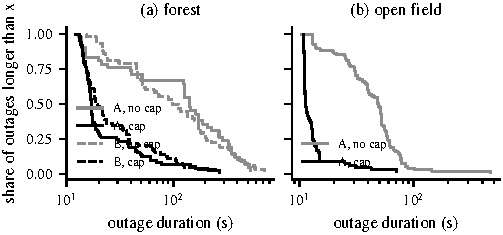
\includegraphics[width=\columnwidth]{fig_outage.pdf}
\caption{Length of C2 outages (time a robot's C2 stayed down), like-for-like
arms with and without the cap, one 90-min run each: share of outages longer
than a given duration. Durations below about 15\,s are not resolved.}
\label{fig:outage}
\end{figure}

The same mechanism may bear on the forest result of our earlier
study~\cite{makhubela2026satnac}, where a roaming node drove 8\,Mb/s video
bursts to over 70\,\% loss; its traffic pattern differed, and we have not
tested this.

\textit{Cap versus 5G-native separation.} A separate network slice or QoS flow
for C2 would also keep C2 out of the video queue, but not shorten the video's
own delay. \todo{slice-per-traffic-class experiment: no cap, cap, slice, slice
+ cap, static forest load test and one patrol}
% E5: tab_a5_patrol; E6: fig_cap_arms (summary CSV, sets xyz/capped)

\begin{figure}[t]
\centering
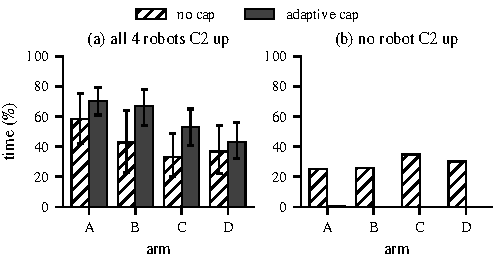
\includegraphics[width=\columnwidth]{fig_cap_arms.pdf}
\caption{Forest fly-off, each placement arm without and with the adaptive cap
(one 90-min run per bar; whiskers: 95\,\% block-bootstrap CI). Arms C and D
used an upper-confidence-bound (UCB) altitude bandit uncapped and the prober
learner capped, so only A and B flew the same policy in both conditions.}
\label{fig:caparms}
\end{figure}


\subsection{C2: Terrain-Blind Forecasting Has Modest Skill, and Capacity Hurts}
\label{sec:r-forecast}

\textit{A linear model forecasts failure onset 20\,s ahead on unseen terrain,
weakly.} After dead-process censoring (Section~\ref{sec:dead}), the best
model, an L1-regularised logistic regression on 65 terrain-blind features,
reaches a pooled PR-AUC 1.79 times the no-skill rate and ROC-AUC 0.667, and no
held-out terrain falls below ROC-AUC 0.538 (Fig.~\ref{fig:capacity}). Skill
peaks at a 20-s horizon: a six-feature trend model scores ROC-AUC 0.650 at
20\,s and 0.552 at 60\,s (Table~\ref{tab:a2}). Forest labels in this data
predate the cap and are partly queue backlog (Section~\ref{sec:r-cap}).
\todo{retrain all eight model classes on the capped, monitor-protected runs and
report beside these numbers}
% A6: phase2c_model_class.csv; A5: phase2b_onset.csv

\begin{figure}[t]
\centering
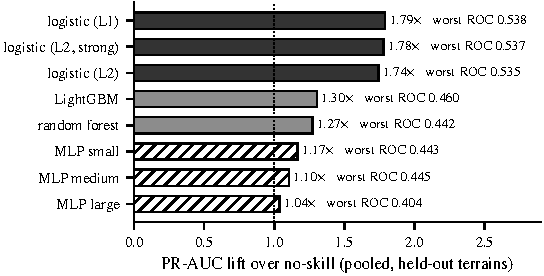
\includegraphics[width=\columnwidth]{fig_capacity.pdf}
\caption{Forecasting skill by model class: pooled PR-AUC lift over no skill
on held-out terrains, and the worst held-out-terrain ROC-AUC (65 features,
20-s onset horizon, 38,303 onset observations, leave-one-terrain-out).}
\label{fig:capacity}
\end{figure}

\textit{More capacity is worse.} On identical folds and features the ordering
is monotone in capacity: three linear models lead, tree ensembles follow, and
three multilayer perceptrons trail. The largest network scores ROC-AUC 0.503,
and 0.404 on its worst terrain, below chance. One exception should be stated:
on six trend features at a 60-s horizon, the medium network beats the linear
models on pooled lift (1.55 against 1.21--1.22) but not on its worst terrain (ROC
0.456 against 0.550). Sequence models on 10\,Hz radio traces add nothing: on
3,115 labelled cycles over three folds, a temporal convolutional network (TCN) and a gated recurrent unit (GRU)
average ROC-AUC 0.493
and 0.523 against 0.540 for a logistic regression on window summaries (A7).
Under leave-one-terrain-out validation with four terrains, we take worst-fold
skill, not pooled skill, as the figure of merit; our reading is that it rewards
models that learn a direction rather than thresholds tied to the training
terrains.
% A6 exception: phase2c n==38803 block, trend6 mlp_medium 1.551 / worst 0.456 vs logistic_L2 1.221 / 0.551; A7: phase6_seq.csv

\subsection{C3: The Model Does Not Recover How Terrain Changes the Altitude Effect}
\label{sec:r-flip}

The measured effect of climbing differs strongly between terrains: per +10\,m,
C2 availability gains 0.208 more in open field than in forest per cycle, and
0.167 more on a uniform 60-s time base that removes the outcome-dependent cycle
length (Table~\ref{tab:contrasts}). This terrain dependence was reported
in~\cite{makhubela2026satnac}; the question here is whether a terrain-blind
model recovers it. To give the model every chance we use a gradient-boosted
tree model (LightGBM), which can represent interactions between altitude and
link state, trained on the same terrain-blind features and held-out terrains.
It does not recover it. At the 20-s horizon of Section~\ref{sec:r-forecast}, the
open-field-minus-forest contrast in the model's risk is $+0.001$ ($p = 0.89$),
and no contrast is significant. At a 60-s horizon it is $+0.006$ ($p = 0.37$),
and two other contrasts are significantly inverted. On coarser 120-s bins one
recovered contrast reaches significance but stays about one sixth of the
measured value (Appendix~\ref{app:tables}).
% C3: tab_contrasts (phase4b_interactions measured/raw h60; phase4b_h20 raw; phase4c 60 s bins); 120 s: phase4d recovered_raw

\begin{table}[t]
\caption{Altitude-Effect Contrasts (C2 Availability per +10\,m): Measured,
and Recovered From a Terrain-Blind LightGBM Model at Two Forecast Horizons.
$^*$: 95\,\% Block-Bootstrap CI Excludes 0}
\label{tab:contrasts}
\centering
\small
\begin{tabular}{@{}c@{}}
{\footnotesize \hspace{16mm}measured\hspace{14mm}recovered}\\[-1pt]
% generated by tab_contrasts.py -- do not edit
\begin{tabular}{@{}lcccc@{}}
\toprule
Contrast & Cycle & 60-s bins & $h{=}20$\,s & $h{=}60$\,s \\
\midrule
Open $-$ forest & $+0.208$$^*$ & $+0.167$$^*$ & $+0.001$ & $+0.006$ \\
Open $-$ hills & $+0.153$$^*$ & $+0.138$$^*$ & $-0.003$ & $+0.037$$^*$ \\
Urban $-$ forest & $+0.073$$^*$ & $+0.070$$^*$ & $+0.006$ & $-0.020$$^*$ \\
Hills $-$ forest & $+0.055$$^*$ & $+0.030$ & $+0.003$ & $-0.031$$^*$ \\
\bottomrule
\end{tabular}
% measured: per cycle and 60-s uniform bins; recovered (LightGBM): per cycle at horizons 20 s and 60 s

\end{tabular}
\end{table}

The consequence for control is direct. Replayed through the planner on each
held-out terrain, no surrogate chooses altitude sensibly: linear models choose
about 55\,m in every terrain, and a gradient-boosted model chooses about 47\,m in both
forest and open field (D1). Altitude therefore has to be learned during the
mission.
% D1: logs/ml/altsel_run.log

\subsection{C4: Learned Placement Under the Cap}
\label{sec:r-place}

\textit{An exploring altitude learner did worse than the baselines in single runs.} With the cap on,
hover (A) and centroid (B) kept all four robots connected 70.5\,\% and
67.0\,\% of the time in forest, indistinguishable from each other (B$-$A
$-4.0$ [$-20.4$, $+11.2$] points). The two arms with an exploring learner were
worse within their runs: C$-$A $-18.1$ [$-34.1$, $-2.6$] and D$-$A $-27.4$
[$-43.0$, $-10.7$]. These are single runs on different nights, and the
night-to-night swings of a same-policy null control reach about 20 points
(Table~\ref{tab:a3}), so the size of the loss is not established. Both
exploring arms spent much of the mission at 45--55\,m (Fig.~\ref{fig:alt}).
% D5: capped summary + CAPPED_FOREST_FLYOFF_REPORT bootstrap table

\textit{One mission cannot determine the sign of the forest altitude effect.}
Comparing arm C with arm B at matched times, with the same x--y rule and
seed, gives $-6.6$ points of C2 per +10\,m ($[-14.9, +0.9]$): probably harmful,
not established, and too small on its point estimate to explain the whole
gap above. The slope the learner itself can estimate within one 90-min
run is $+4.6$ ($[-9.1, +12.0]$) in arm C and $+5.9$ ($[-10.7, +14.9]$) in arm
D. Its interval spans both signs, so the learner moved on noise.
% D6: logs/ml/forest_altitude_effect_capped.csv

\begin{figure*}[t]
\centering
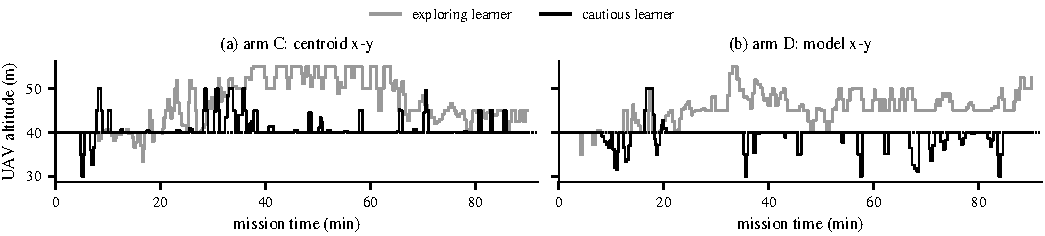
\includegraphics[width=\textwidth]{fig_altitude.pdf}
\caption{UAV altitude during the capped forest missions for the two
learned-altitude arms. The exploring learner drifts to 45--55\,m; the cautious
learner keeps 40\,m as its incumbent and leaves it only for short probes.}
\label{fig:alt}
\end{figure*}

\textit{A cautious learner behaves like hover.} Homed at 40\,m and requiring 1.5 standard
errors plus 0.02 of reward to move away, the learner kept 40\,m as its
incumbent in both arms and spent 83--84\,\% of each mission there. All four
robots were connected 65.2\,\% (C) and 72.0\,\% (D) of the time, not
distinguishable from the baselines, though the intervals are wide (C$-$A
$-5.1$ [$-17.9$, $+6.8$]; D$-$A $+1.6$ [$-13.4$, $+17.7$]),
and arm D scored $+28.8$ [$+11.9$, $+45.1$] points above its exploring version,
again a cross-night single-run comparison. In effect the cautious learner is
hover with short probes: it gave no benefit over hover. No learned arm beat a
baseline. \todo{replace with the 3-seed forest and
open-field results of the repeat campaign (Fig.~\ref{fig:seeds}); decision rule
fixed in CLAIMS.md}
% D7: cautious_forest_flyoff summary; time at 40 m: flyoff_forest_cautious_analyse.py

\begin{figure}[t]
\centering
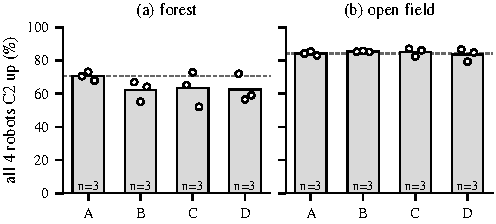
\includegraphics[width=\columnwidth]{fig_arms_seeds.pdf}
\caption{All four robots C2 up per arm with the cap, cautious learner for C
and D; bar = mean over runs, dots = individual 90-min runs. \todo{partial:
forest seed 1 only; regenerate after the repeat campaign}}
\label{fig:seeds}
\end{figure}

\textit{The risk planner survives its null control in open field only.}
Against the repositioning policy of~\cite{makhubela2026satnac}, matched on
geometry, the planner gained $+10.5$ [$+7.0$, $+13.2$] points in open field.
The same comparison between two nights of the \emph{same} baseline policy gave
$-0.5$ [$-4.3$, $+3.0$] there, which rules out a night-to-night swing of that
size, so the gain is interpretable. In forest the planner lost $-15.3$
[$-24.8$, $-5.0$], but the null control's interval [$-17.6$, $+6.4$] admits a
swing that large; in urban and hills the null was itself as large as the
effect ($+18.7$ and $-21.7$). Those three comparisons are uninterpretable
(Table~\ref{tab:a3}).
% C2: planner_vs_twophase_nullctl.csv
